$k$-nearest Neighbor was put forward by Cover and Hart in 1968\cite{knn}, is a classification algorithm, which is supervised and non-parametric. The problem, which K-NN solves, can be described as follows.

	  Given a labeled set $T=\{(x_i,y_i)|x_i\in\mathbb{R}^n, y_i\in C, i=1,2,\dots,N\}$, where $C$ is the set of categories, $C=\{c_1,c_2,\dots,c_s\}$. We need to find out the category of the new instance, $x$. We will denote $y$ as the category of $x$.

%	We will define ``neighbor" i.

\section{How to Define ``Neighbor"}
	To define ``neighbor", we introduce the definition of distance metrics in $\mathbb{R}^n$ firstly.
%	Because the labeled data instance $x_i\in\mathbb{R}^n$, here we only introduce the distance metrics in European space, $\mathbb{R}^n$.

	\begin{definition}
	Assume that $x_i, x_j\in\mathbb{R}^n$, and note that
	$$x_i=(x_i^{(1)},x_i^{(2)},\dots,x_i^{(n)})$$
		$$x_j=(x_j^{(1)},x_j^{(2)},\dots,x_j^{(n)})$$
		Then we define $L_p$ distance
		\begin{equation}
		L_p(x_i, x_j):=(\sum_{l=1}^{n} |x_i^{(l)}-x_j^{(l)}|^p)^{\cfrac{1}{p}}, p\geq 1
		\end{equation}

		i.e. when $p=2$, this distance is Euclidean distance,
		\begin{equation}
		L_2(x_i, x_j):=(\sum_{l=1}^{n} |x_i^{(l)}-x_j^{(l)}|^2)^{\cfrac{1}{2}}
		\end{equation}

	%	If $p=1$, it is Manhattan distance,
	%	\begin{equation}
	%	L_1(x_i, x_j):=\sum_{l=1}^{n} |x_i^{(l)}-x_j^{(l)}|
	%	\end{equation}

	%	If $p=\infty$, it is The maximum value of each coordinate distance,
	%	\begin{equation}
	%	L_{\infty}(x_i,x_j):=\max_{l} |x_i^{(l)}-x_j^{(l)}|
	%	\end{equation}
         \end{definition}

	    The figure \ref{alo:distance} shows that the points whose distance from the origin is 1 in $\mathbb{R}^n$.
	    \begin{figure}[htbp]
	    	\centering{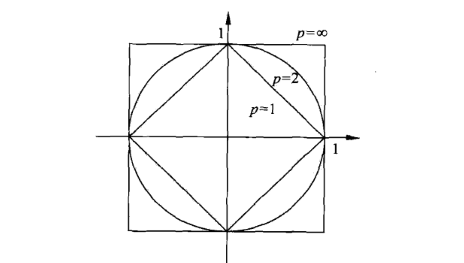
\includegraphics[width=10cm]{distance.png}}
	    	\caption{Relationship between the different $L_p$ distance}
	    	\label{alo:distance}
	    \end{figure}

    Now we can define ``neighbor", i.e., given $p$, the nearest neighbor of $x_i$ is the point that has the minimal $L_p$ distance to $x_i$. It is worthy to note that the nearest neighbor determined under different distance metrics are generally different.

\section{$k$-NN Algorithm}

       $k$-NN predicts category of $x$ via the following Algorithm.

	\begin{algorithm}
    	\caption{$k$-NN}
    	\label{alo:K-NN}
    	\textbf{Input:}  Set $T=\{(x_i, y_i)|x_i\in\mathbb{R}^n, y_i\in C, i=1,2,\dots,N\}$, $x$ and $k$, where $C = \{c_{1}, c_{2}, \dots, c_{s}\}$. \\
    	\textbf{Output:} $y$ (the category of $x$)

    	\begin{algorithmic}[1]
         \State Find $k$ neighbors $x_j\in T, j=i_1,\dots,i_k$, i.e.
    	 \begin{align*}
    	 x_{i_1}&={\arg\min}_{x_i\in T} \|x-x_i\|_2,\\
    	 x_{i_m}&={\arg\min}_{x_i\in T\setminus \{\cup_{n<m}x_{i_n}\}} \|x-x_i\|_2, 1<m\leq k
    	 \end{align*}
    	 \State Define $y$ is the category of $x$,and find out it. $$y={\arg\max}_{c_l}\sum_{j=i_1,\cdots,i_k}I(y_j=c_l), l=1,2,\dots,s$$ where I is instruction function, that is, if $y_j=c_l$, then $I=1$, or $I=0$.
    	\end{algorithmic}
    \end{algorithm}

	\textbf{Shortcomings of $k$-NN}:
	  \begin{enumerate}
	  	\item It is sensitive to the local structure of the data, easy to over-fit the data.
	  	\item It is expensive to calculate the distance each time. 
	  \end{enumerate}
	  
	  To cut down the expense of computation, one classical method is the $\textbf{$k$-d tree}$(short for $k$-dimensional tree), where the $k$ is different with the $k$ used by above $k$-NN. In computer science, a $k$-d tree is a space-partitioning data structure for organizing points in a $k$-dimensional space. Next we introduce how to construct one $k$-d tree, which can represent and store the distance relation between points.
	  
	 \begin{algorithm}
    	\caption{Construct Balanced $k$-d Tree}
    	\label{alo:kdtree}
    	\textbf{Input:} Set $T=\{x_i | x_i\in\mathbb{R}^k, i=1,2,\dots,N\}$, where $x_{i} = (x_{i}^{(1)}, x_{i}^{(2)}, \dots, x_{i}^{(k)})$. \\
    	\textbf{Output:} $k$-d Tree

    	\begin{algorithmic}[1]
	\State Find one rectangle region $\mathscr{R}_{0}$ to cover set $T$, i.e.
	\[\mathscr{R}_{0} = \{x| \min_{i} x_{i}^{(j)} < x^{(j)} < \max_{i} x_{i}^{(j)}\}\]
         Define $\mathscr{R}_{0}$ as the root node with $0$-depth. 

    	 \State \textbf{Repeat}: for $m$-th $j$-depth node and $l = (j \ mod \ k) + 1$, 
	 
	 \begin{enumerate}[a]
	 \item If $\# (T \cap  \mathscr{R}_{j}^{m}) \nmid 2$,  
	 $$ i_{0} = \arg median_{i}\{ x_{i}^{(l)}\}$$
	 
	 use the hyperplane $x^{(l)} = x_{i_{0}}^{(l)}$ to divide $\mathscr{R}_{j}^{m}$ into two subregions as $\mathscr{R}_{j + 1}^{2m-1}$ and $\mathscr{R}_{j + 1}^{2m}$. Then store $x_{i_{0}}$ in the node $\mathscr{R}_{j}^{m}$.
	 
	 \item If $\# (T \cap  \mathscr{R}_{j}^{m}) \mid 2$ and $\# (T \cap  \mathscr{R}_{j}^{m}) \neq 0$, 
	 $$ \hat{x}^{(l)} = median_{i}\{ x_{i}^{(l)}\}$$
	 
	 similarly, the hyperplane $x^{(l)} = \hat{x}^{(l)}$ to divide $\mathscr{R}_{j}^{m}$ into two subregions as $\mathscr{R}_{j + 1}^{2m-1}$ and $\mathscr{R}_{j + 1}^{2m}$.
	 
	 \item If $\# (T \cap  \mathscr{R}_{j}^{m}) \mid 2$ and $\# (T \cap  \mathscr{R}_{j}^{m}) = 0$, no partition will be exceeded.
	 
	 Collect all $\mathscr{R}_{j + 1}^{l}$ to get (j + 1)-depth nodes.
  	 \end{enumerate}
	 \textbf{Stop} until 
	 \[ \sum_{m} \# (T \cap  \mathscr{R}_{j + 1}^{m}) = 0 \]
    	\end{algorithmic}
    \end{algorithm}
    
    Now we import an example using $k$-d tree on 2-d set to show the specific details of $\textbf{Algorithm} \  \ref{alo:kdtree}$. 
    
    Given the set $T = \{x_{i}| i = 1: 7\} = \{(1, 1), (1, 5), (2, 9), (3, 3), (5, 2), (6, 7), (8, 4)\}$(Fig $\ref{alo:kdtree}$) as following. At the very beginning, we choose the 1-th coordinate to get the first partition plane $x_{1} = 3$ for the reason that the median of $\{1, 1, 2, 3, 5, 6, 8\}$ is 3. Here we left the following details to our reader to complete the whole algorithm. The $k$-d tree can be drown as one visual tree%(Fig $\ref {alo:kdtree}$).
    
    %%%
    
	\begin{figure}[htbp]
	\centering{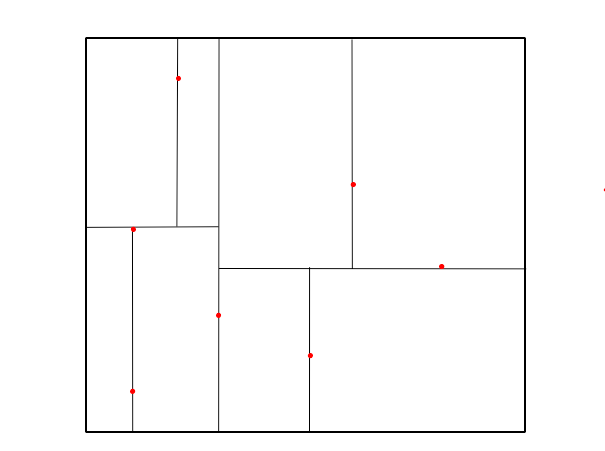
\includegraphics[width=10cm]{kdtree.png}}
	\caption{Result of $k$-d Tree}
	\label{alo:kdtree}
	\end{figure}
    %%%%%%%%%%%%


%%%%%%%%%%%
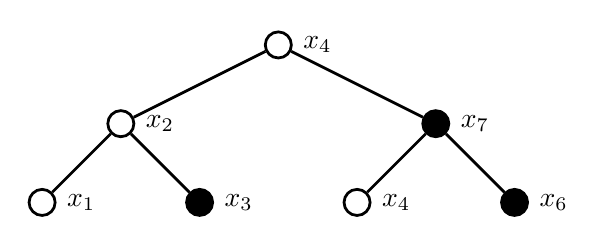
\begin{tikzpicture}[line width = 1pt,
                    solid/.style = {circle, draw, fill = black, minimum size = 0.3cm},
                    empty/.style = {circle, draw, fill = white, minimum size = 0.3cm}]
%%%%%

\node [empty, label = right:$x_4$] (A) at (4,2) {};
\node [empty, label = right:$x_{2}$] (B) at (2,1) {};
\node [solid, label = right:$x_{7}$] (C) at (6,1) {};
\node [empty, label = right:$x_{1}$] (D) at (1,0) {};
\node [solid, label = right:$x_{3}$] (E) at (3,0) {};
\node [empty, label = right:$x_{4}$] (F) at (5,0) {};
\node [solid, label = right:$x_{6}$] (G) at (7,0) {};

\draw (A) -- (B);
\draw (A) -- (C);
\draw (B) -- (D);
\draw (B) -- (E);
\draw (C) -- (F);
\draw (C) -- (G);


\end{tikzpicture}





    
    $k$-d tree can save lots of computation in $k$-NN. We briefly give the recipe of $k$-d tree method of finding the nearest neighbor of one new instance, $x$.
    
    	 \begin{algorithm}
    	\caption{Using $k$-d Tree to Find the Nearest Neighbor}
    	\label{alo:kdtree}
    	\textbf{Input:} $k$-d tree of data set and new instance, $x$ \\
    	\textbf{Output:} Nearest neighbor

    	\begin{algorithmic}[1]
	\State Find the leaf node that contains $x$.
	
	\textbf{Downward retrieval}: from the root node, according to information stored in the nodes, such as the corresponding partition hyperplane, to move our searching road to next depth right or left child node. Repeat the above process until arriving one leaf node, say $x^{*}$, which named as the current nearest neighbor.
	
	\State{\textbf{Upward check and Repeat}}: for one current nearest neighbor, $x^{*}$, whose depth is j,
	
	\begin{enumerate}[(1)]
	\item Compute 
	$$d(x^{*}, x) = ||x^{*} - x||$$
	\item Backward to $x^{*}$'s parent node, say $x_{j - 1}$. 
	\item Check the other child node of $x_{j - 1}$, say $x^{**}$, if $d(x^{**}, x) \leq d(x^{*}, x) $, let $x^{*} = x^{**}$.
	\end{enumerate}
	 
         \textbf{Stop}: j = 0. 
    	\end{algorithmic}
    \end{algorithm}
    
	   

\section{The Choice of Parameter $k$}
    The choice of $k$ has significant impact on the results of $k$-NN.

    If we choose a smaller $k$, the forecast results are usually very sensitive to the neighboring instance points. In particular, the neighboring instance points may be noise. For one exact example, we have one labeled set in $\mathbb{R}^{2}$, which has two categories drawn in colors, `green' and `blue', and one red instance waiting its category. It's obvious that the red instance should better be grouped into the green class. When choosing a small $k$, we will get the bad result, `blue'.  By contrast, choosing a larger $k$, the labeled instances, which are distant from the target, will make unnecessary contribution. Then $k$-NN will be fail again. As the figure $\ref{alo: large k}$ shows, if we select the whole labeled points, then we will get category `blue' instead of `green'.

	\begin{figure}[htbp]
	    \centering{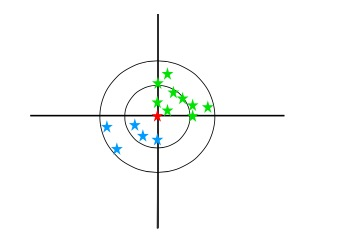
\includegraphics[width=10cm]{small_k.png}}
	    \caption{One example of choosing a smaller $k$}
	    \label{alo:small k}
        \end{figure}


   

       \begin{figure}[htbp]
	\centering{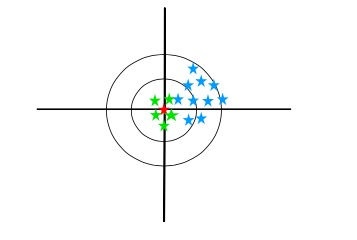
\includegraphics[width=10cm]{large_k.png}}
	\caption{One example of choosing a larger $k$}
	\label{alo: large k}
       \end{figure}



    In general, the choice of $k$ depends on the data. One can use Cross-Validation method to find an optimal $k$.

    \begin{algorithm}
    	\caption{Find the Optimal $k$}
    	\label{alo:find the optimal k}
    	\textbf{Input:}  labeled set $D=\{(x, y)|x \in\mathbb{R}^n, y \in C, i=1,2,\dots, N\}$, where $C = \{c_{1}, c_{2}, \dots, c_{s}\}$.\\
    	\textbf{Output:} $k$

    	\begin{algorithmic}[1]
         \State Divide data from $D$ into two parts: labeled set $T$ and validation set $Y$, i.e., which are noted as follows,   	 $$T = \{(x_{i}, y_{i})|x_{i} \in\mathbb{R}^{n}, y_{i} \in C, i = 1, 2, \dots, N_{1}\}$$
         $$Y = \{(\hat{x}_{j}, \hat{y}_{j})|\hat{x}_{j} \in\mathbb{R}^{n}, \hat{y}_{j} \in C, j = 1, 2, \dots, N_{2}\}$$
    	 \State Initialize $k = 2$. For $j = 1, 2, \dots, N_{2}$, use the Algorithm $k$-NN on labeled set $T$, then get category label $\tilde{y}_{j}$.\\
	 Define $O^{k}$,
	 $$O^{k} = \sum_{j = 1}^{N_{2}} I(\tilde{y}_{j} = \hat{y}_{j})$$
	 Update $k = k + 1$
    	 \State Stop until $k = N$,
	 $$k = {\arg\max}_{k} O^{k}$$
    	\end{algorithmic}
    \end{algorithm}

